\documentclass[11pt]{article}

\usepackage[a4paper,margin=2.4cm]{geometry}
\usepackage{amsmath, amssymb, mathtools}
\usepackage{amsthm}
\usepackage{booktabs}
%\usepackage{microtype}
\usepackage{tikz}
\usetikzlibrary{calc, arrows.meta, positioning, decorations.pathreplacing}
\usepackage[dvipsnames]{xcolor}
\usepackage{enumitem}
\usepackage{titlesec}
\usepackage{fancyhdr}
\usepackage{hyperref}
\hypersetup{colorlinks=true, linkcolor=NavyBlue, urlcolor=NavyBlue, citecolor=NavyBlue,
  pdftitle={BinMoments --- Mathematical Companion},
  pdfauthor={Dragan Solarov},
  pdfsubject={Additive statistics, Wasserstein distance, and Mahalanobis distance}}

\definecolor{ink}{HTML}{1A2330}
\definecolor{accent}{HTML}{2C5F8A}
\definecolor{soft}{HTML}{5A6B7B}
\definecolor{rulegrey}{HTML}{C8D0D8}
\definecolor{panel}{HTML}{F2F5F8}

\color{ink}

\titleformat{\section}{\Large\bfseries\color{accent}}{\thesection}{0.7em}{}
\titleformat{\subsection}{\large\bfseries\color{ink}}{\thesubsection}{0.6em}{}
\titlespacing{\section}{0pt}{1.6em}{0.7em}

\newtheorem{theorem}{Theorem}
\newtheorem{lemma}{Lemma}
\newtheorem{proposition}{Proposition}
\theoremstyle{definition}
\newtheorem{definition}{Definition}
\newtheorem{remark}{Remark}

\pagestyle{fancy}
\fancyhf{}
\fancyhead[L]{\small\color{soft}BinMoments — Mathematical Companion}
\fancyhead[R]{\small\color{soft}\thepage}
\renewcommand{\headrulewidth}{0.4pt}

\newcommand{\R}{\mathbb{R}}
\newcommand{\E}{\mathbb{E}}
\newcommand{\ind}{\mathbb{1}}
\newcommand{\powsum}{\mathbf{S}}
\newcommand{\fvec}{\mathbf{f}}
\newcommand{\Cov}{\boldsymbol{\Sigma}}
\newcommand{\given}{\,\middle|\,}

% Panel for key results
\usepackage{tcolorbox}
\tcbset{
  keybox/.style={
    colback=panel, colframe=accent, boxrule=0.6pt, arc=2pt,
    left=8pt, right=8pt, top=6pt, bottom=6pt, fonttitle=\bfseries
  }
}

\begin{document}

\begin{center}
  {\LARGE\bfseries\color{accent} BinMoments — Mathematical Companion}\\[0.6em]
  {\large The mathematics the architecture grew from}\\[0.9em]
  {\large\color{ink} Dragan Solarov}\\[1.0em]
  {\color{soft}\rule{0.5\textwidth}{0.4pt}}\\[0.8em]
  {\small Architecture by the author; implementation AI-assisted.\\
  This document records the mathematical foundations: the algebra of additive statistics,\\
  the geometry of distribution distance, and the statistics of vector comparison.}
\end{center}

\vspace{1.2em}

\section*{Where it began}
\addcontentsline{toc}{section}{Where it began}

Every other document in this project describes a system that was \emph{built}. This one describes
the mathematics that the system was built \emph{to serve} --- because the project started from the
mathematics, not the architecture. The seed was a single conviction: that the behaviour of a sensor
can be captured by the \emph{moments} of its value distribution, that those moments can be tracked
\emph{exactly} and combined \emph{cheaply}, and that change in behaviour is best measured as a
\emph{distance between distributions}. Everything else --- the bins, the two clocks, the medallion
layers, the platform --- is that conviction made operational.

This companion answers the three mathematical questions on which the whole design rests:

\begin{enumerate}[leftmargin=1.4em, itemsep=0.3em]
  \item \textbf{Why are the summary statistics additive,} and why does that one property let us
        merge across time and distribute across machines --- while the median cannot? (\S1)
  \item \textbf{Why is the Wasserstein distance} the right way to measure that an instrument's
        distribution has drifted, compared with PSI, KL, Jensen--Shannon, Kolmogorov--Smirnov, and
        cosine? (\S2)
  \item \textbf{Why is the Mahalanobis distance} the appropriate tool for comparing the
        fingerprint \emph{vectors} we may build on in future, and why is it better suited to
        anomaly scoring than nearest-neighbour / ANN search? (\S3)
\end{enumerate}

A single thread runs through all three: \emph{additivity}. The statistics we keep are sums of
per-element functions; sums merge; and that algebraic fact is what makes the system reproducible,
distributable, and --- in \S3 --- extensible.

\section{Additive sufficient statistics: the power-sum vector}

\subsection{The object we actually store}

We never store raw readings as the summary. For each instrument--channel--hour we store a short
vector of \emph{power sums}. Given values $x_1, \dots, x_n$ (the readings in one bucket),

\begin{equation}
  \powsum \;=\; \bigl(S_0,\, S_1,\, S_2,\, S_3,\, S_4\bigr),
  \qquad
  S_k \;=\; \sum_{i=1}^{n} x_i^{\,k},
\end{equation}

so $S_0 = n$ (the count), $S_1 = \sum x_i$, $S_2 = \sum x_i^2$, and so on. Five numbers, regardless
of how many readings landed in the bucket. From these we recover the \emph{raw moments}
$m_k' = S_k / n$ and then the central moments and the shape statistics. The claim of this section
is that this little vector is exactly the right thing to keep: it is \emph{sufficient} for the
moments, and --- crucially --- it is \emph{additive}.

\subsection{The additivity theorem}

\begin{theorem}[Additivity of power sums]\label{thm:add}
Let $A$ and $B$ be two disjoint collections of readings, and let $A \uplus B$ be their combined
collection. Then
\begin{equation}
  \powsum(A \uplus B) \;=\; \powsum(A) \;+\; \powsum(B),
\end{equation}
where the addition on the right is ordinary componentwise vector addition.
\end{theorem}

\begin{proof}
Fix any order $k \in \{0,1,2,3,4\}$. By the definition of the power sum and the fact that summing
over a disjoint union is summing over each part and adding,
\begin{equation}
  S_k(A \uplus B)
  \;=\; \sum_{x \in A \uplus B} x^{k}
  \;=\; \sum_{x \in A} x^{k} \;+\; \sum_{x \in B} x^{k}
  \;=\; S_k(A) + S_k(B).
\end{equation}
This holds for every component $k$ simultaneously, which is precisely componentwise vector
addition. \qed
\end{proof}

The proof is almost trivial --- and that triviality is the point. The reason it works is structural:
each power sum is a \textbf{sum of a function applied to each element}, $S_k = \sum_i \phi_k(x_i)$
with $\phi_k(x) = x^k$. Any statistic of that form decomposes over a disjoint union, because the
elements of $A$ and the elements of $B$ are simply different terms in one big sum. We will see in
\S1.4 that the median has \emph{no} such form, and that this is exactly why it cannot be merged.

\subsection{The algebraic structure: a commutative monoid}

Theorem~\ref{thm:add} says more than ``you can add them.'' It says the map

\begin{equation}
  A \;\longmapsto\; \powsum(A) \in \R^5
\end{equation}

is a homomorphism from the collection of datasets (under disjoint union $\uplus$) into the additive
group $(\R^5, +)$. Concretely, the merge operation $\oplus$ on stored summaries is just vector
addition, and it inherits two properties from $+$:

\begin{itemize}[leftmargin=1.4em, itemsep=0.2em]
  \item \textbf{Associativity:} $(\powsum_A \oplus \powsum_B) \oplus \powsum_C
        = \powsum_A \oplus (\powsum_B \oplus \powsum_C)$.
  \item \textbf{Commutativity:} $\powsum_A \oplus \powsum_B = \powsum_B \oplus \powsum_A$,
        with identity element $\mathbf{0}$ (the empty bucket).
\end{itemize}

A set with an associative, commutative operation and an identity is a \emph{commutative monoid}.
This is the precise algebraic reason the architecture can do what it does:

\begin{tcolorbox}[keybox, title={Why the algebra matters}]
Because merging summaries is an associative, commutative operation, partial summaries can be
combined \textbf{in any order and in any grouping} and still yield the same result. That is exactly
what is required to (i) accumulate a running total over a bitemporal, append-only history
(\emph{merge across time}), and (ii) compute partial sums on many machines and combine them
(\emph{merge across space}). The same property delivers both. The choice was made for
reproducibility; distribution came free.
\end{tcolorbox}

\begin{center}
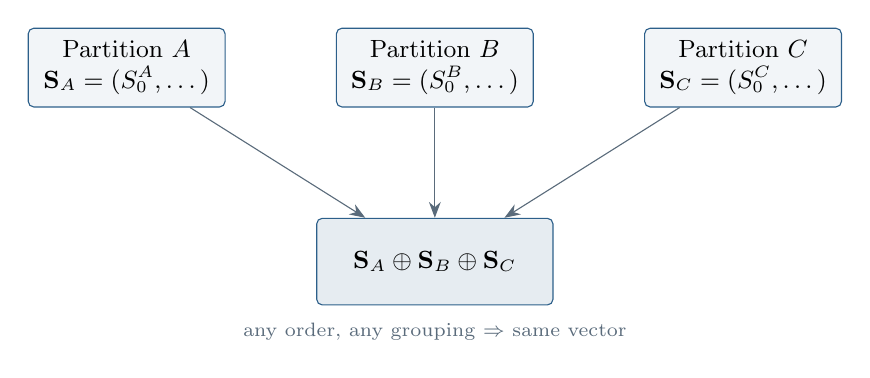
\begin{tikzpicture}[font=\small, node distance=6mm]
  \tikzset{
    part/.style={draw=accent, fill=panel, rounded corners=2pt, minimum width=2.5cm, minimum height=1.0cm, align=center},
    merged/.style={draw=accent, fill=accent!12, rounded corners=2pt, minimum width=3.0cm, minimum height=1.1cm, align=center, font=\small\bfseries}
  }
  \node[part] (a) {Partition $A$\\$\powsum_A=(S_0^A,\dots)$};
  \node[part, right=1.4cm of a] (b) {Partition $B$\\$\powsum_B=(S_0^B,\dots)$};
  \node[part, right=1.4cm of b] (c) {Partition $C$\\$\powsum_C=(S_0^C,\dots)$};
  \node[merged, below=1.4cm of b] (m) {$\powsum_A \oplus \powsum_B \oplus \powsum_C$};
  \draw[-{Stealth[length=2mm]}, soft] (a) -- (m);
  \draw[-{Stealth[length=2mm]}, soft] (b) -- (m);
  \draw[-{Stealth[length=2mm]}, soft] (c) -- (m);
  \node[below=1mm of m, soft, font=\scriptsize] {any order, any grouping $\Rightarrow$ same vector};
\end{tikzpicture}
\end{center}

\subsection{From power sums to moments (exactly)}

The power-sum vector is \emph{sufficient} for the central moments: every moment we report is a
deterministic function of $\powsum$, computed exactly (no binning, no approximation). With
$\mu = m_1' = S_1/n$ and raw moments $m_k' = S_k/n$, the central moments follow from the binomial
expansion $\mu_k = \E[(X-\mu)^k] = \sum_{j=0}^{k}\binom{k}{j}(-1)^{k-j} m_j' \,\mu^{\,k-j}$:

\begin{align}
  \text{mean}      \quad &\mu   = \tfrac{S_1}{n}, \\[0.2em]
  \text{variance}  \quad &\mu_2 = m_2' - \mu^2, \\[0.2em]
  \text{3rd central}\quad &\mu_3 = m_3' - 3\mu\, m_2' + 2\mu^3, \\[0.2em]
  \text{4th central}\quad &\mu_4 = m_4' - 4\mu\, m_3' + 6\mu^2 m_2' - 3\mu^4,
\end{align}

and the standardised shape statistics are

\begin{equation}
  \text{skewness}\;\; \gamma_1 = \frac{\mu_3}{\mu_2^{3/2}},
  \qquad
  \text{excess kurtosis}\;\; \gamma_2 = \frac{\mu_4}{\mu_2^{2}} - 3.
\end{equation}

\begin{remark}[Why this beat reading moments off the bins]
An earlier version of the design computed moments from the histogram bin midpoints with a
Sheppard-type correction. Numerical validation refuted it: with \emph{equal-mass} bins the tail
bins are very wide, so a bin's midpoint is a poor stand-in for where its mass actually sits, and the
variance was overestimated by 5--90\% depending on bin count (higher moments worse, since they
weight the tails by $x^3$ and $x^4$). The power-sum route above has \emph{no} such bias: it is the
exact moment of the data, and it is additive, so nothing was given up to get exactness. Bins were
kept for what they are genuinely good at --- percentiles and entropy (\S1.5).
\end{remark}

\begin{remark}[A note on numerical care]
Computing $\mu_2 = m_2' - \mu^2$ as a difference of two large nearly-equal numbers can lose
precision (catastrophic cancellation) when the mean is large relative to the spread. In practice
this is mitigated by accumulating sums about a provisional mean (a shifted/centered form) or by
the streaming covariance updates of Welford/Chan, which are themselves additive and merge by the
same monoid law. The algebra of \S1.2 is unaffected; only the floating-point bookkeeping changes.
\end{remark}

\subsection{What is \emph{not} additive --- and why}

Not every useful statistic can be stored and merged this way. The clearest example is the median.

\begin{proposition}[The median does not merge from medians]\label{prop:median}
There is no function $h$ such that $\operatorname{med}(A \uplus B) = h\bigl(\operatorname{med}(A),
\operatorname{med}(B)\bigr)$ for all datasets $A, B$.
\end{proposition}

\begin{proof}
It suffices to exhibit two pairs with \emph{equal} component medians but \emph{different} merged
medians; then no function of the component medians could return both answers. Take
\begin{align*}
  A  &= \{1, 2, 3\}, & B  &= \{4, 5, 6\}, & &\operatorname{med}(A)=2,\ \operatorname{med}(B)=5, \\
  A' &= \{0, 2, 100\}, & B' &= \{3, 5, 7\}, & &\operatorname{med}(A')=2,\ \operatorname{med}(B')=5.
\end{align*}
Then $A \uplus B = \{1,2,3,4,5,6\}$ has median $3.5$, while $A' \uplus B' = \{0,2,3,5,7,100\}$ has
median $4$. The inputs to any candidate $h$ are identical ($2$ and $5$) yet the required outputs
differ ($3.5 \neq 4$). No such $h$ exists. \qed
\end{proof}

The deep reason mirrors \S1.2. The median is a function of the \emph{order statistics} --- it asks
``which value sits in the middle once everything is sorted?'' --- and sorting cannot be written as
$\sum_i \phi(x_i)$ for any fixed per-element function $\phi$. The contribution of a reading to the
median depends on \emph{all the other readings}, not on the reading alone. The same holds for the
mode, the exact quantiles, and the minimum and maximum (which are merge\emph{able} but by
$\max/\min$, not by addition --- a different monoid).

\subsection{The resolution: keep additive carriers, derive everything from them}

If the median is not additive, how do we report percentiles at all? The answer is that we keep a
\emph{second} additive object --- the histogram bin counts --- and read order-based statistics from
it to controlled resolution. For fixed bin edges defining bins $b = 1, \dots, B$, the count vector is

\begin{equation}
  \mathbf{c} = (c_1, \dots, c_B),
  \qquad
  c_b = \sum_{i=1}^{n} \ind\!\left[x_i \in \text{bin } b\right].
\end{equation}

Each $c_b$ is again a \emph{sum of a per-element function} (an indicator), so by the identical
argument as Theorem~\ref{thm:add} the count vector is additive: $\mathbf{c}(A \uplus B)
= \mathbf{c}(A) + \mathbf{c}(B)$. From the merged counts we obtain:

\begin{itemize}[leftmargin=1.4em, itemsep=0.25em]
  \item \textbf{Percentiles} (including a median estimate) by walking the cumulative counts to the
        desired mass and interpolating within the bin --- exact to bin resolution, which the
        equal-mass scheme places where the data actually lives.
  \item \textbf{Entropy} $H = -\sum_b p_b \log p_b$ with $p_b = c_b / n$.
\end{itemize}

\begin{tcolorbox}[keybox, title={Additive vs.\ derived --- the distinction that organises everything}]
A statistic being \emph{additive} ($T(A\uplus B)=T(A)+T(B)$) is different from a statistic being
\emph{derivable from additive carriers}. Variance, skewness, kurtosis, percentiles, and entropy are
\textbf{not} additive --- you cannot add two variances or two entropies. But every one of them is a
deterministic function of objects that \emph{are} additive: the power-sum vector $\powsum$ and the
count vector $\mathbf{c}$. So we store the additive carriers, merge those freely across time and
machines, and compute the reported statistics on demand. The only thing genuinely out of reach is a
statistic requiring exact global order (the true median), which we replace with its histogram
estimate.
\end{tcolorbox}

\subsection{One object: the fingerprint}

Finally, the reported summaries are collected into a single vector --- the \emph{fingerprint} of an
instrument--hour:

\begin{equation}
  \fvec = \bigl(\,\mu,\; \mu_2,\; \gamma_1,\; \gamma_2,\;
  q_{50},\, q_{90},\, q_{95},\, q_{99},\; H_{\text{norm}}\,\bigr) \in \R^9 .
\end{equation}

It is worth being clear about the two layers here. The fingerprint $\fvec$ is the \emph{derived,
reported} object --- the thing a human or a downstream model looks at. The power-sum vector
$\powsum$ and the count vector $\mathbf{c}$ are the \emph{stored, additive carriers} from which
$\fvec$ is computed. We merge at the carrier layer (where addition is valid) and compare at the
fingerprint layer (\S3). Keeping these straight is what lets the system be both mergeable and
expressive at once.


\section{Comparing distributions: why Wasserstein}

\subsection{The question, stated precisely}

Drift detection asks: \emph{has this instrument's value distribution moved away from its own
normal?} Formally, let $F$ be the cumulative distribution function (CDF) of a recent window of
readings and $G$ the CDF of a baseline (the instrument's calibrated normal). We need a number
$D(F, G)$ that is small when the two distributions agree and grows as they diverge --- and, for an
operator to trust it, that number should mean something. The choice of $D$ is not cosmetic: different
distances are sensitive to different kinds of change, and several common choices are blind to
exactly the change we care about.

\subsection{The Wasserstein-1 distance}

\begin{definition}[Wasserstein-1, one dimension]
For distributions on $\R$ with CDFs $F$ and $G$,
\begin{equation}
  W_1(F, G)
  \;=\; \int_{-\infty}^{\infty} \bigl| F(x) - G(x) \bigr|\, dx
  \;=\; \int_{0}^{1} \bigl| F^{-1}(u) - G^{-1}(u) \bigr|\, du .
\end{equation}
\end{definition}

The two forms are equal in one dimension and each tells a story. The first integrates the
\emph{horizontal} gap between the CDF curves (the area between them). The second integrates the gap
between the \emph{quantile functions} $F^{-1}, G^{-1}$: it is the average distance each unit of
probability mass must travel to turn one distribution into the other --- which is why $W_1$ is also
called the \emph{earth mover's distance}. Mass is dirt; $W_1$ is the least work to reshape one pile
into the other.

Three properties make it the right primary signal:

\begin{enumerate}[leftmargin=1.5em, itemsep=0.3em]
  \item \textbf{It is a true metric.} $W_1(F,G) \ge 0$ with equality iff $F = G$; it is symmetric;
        and it satisfies the triangle inequality $W_1(F,H) \le W_1(F,G) + W_1(G,H)$. Distances that
        violate these (see KL, PSI below) are harder to reason about and to threshold.
  \item \textbf{It is in the units of the measurement.} $W_1$ is measured in degrees Celsius, not in
        a dimensionless divergence. A drift of ``$W_1 = 3.3$'' \emph{means} the distribution moved
        by about $3.3^\circ$C of mass-transport --- directly interpretable, directly thresholdable.
  \item \textbf{It respects the geometry of the value axis (ground distance).} Moving mass to an
        adjacent bin costs little; moving it far costs a lot. Bin-wise divergences (\S2.4) cannot see
        this --- to them, any change of bin is equally large.
\end{enumerate}

\subsection{The shift property (a clean sanity check)}

\begin{proposition}[A pure shift costs exactly its size]
If $G$ is $F$ shifted by a constant $\delta$ (i.e.\ the readings all move by $\delta$), then
$W_1(F, G) = |\delta|$.
\end{proposition}

\begin{proof}
A shift by $\delta$ sends each quantile to $G^{-1}(u) = F^{-1}(u) + \delta$. Using the quantile form,
\begin{equation}
  W_1(F, G) = \int_0^1 \bigl| F^{-1}(u) - \bigl(F^{-1}(u) + \delta\bigr) \bigr|\, du
            = \int_0^1 |\delta|\, du = |\delta| . \qquad\qed
\end{equation}
\end{proof}

This is the property that makes the detector legible. The simulated $+4^\circ$C fault produced
day-distances near $3.3^\circ$C (a little under $4$, because each day mixes drifted and undrifted
hours), against a self-calibrated quiet-day threshold near $1.7^\circ$C --- numbers an engineer can
read directly as ``the distribution moved by about three degrees.''

\begin{center}
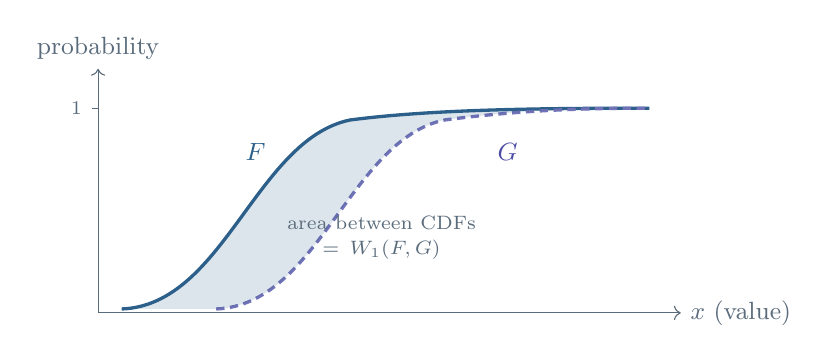
\begin{tikzpicture}[scale=1.0, font=\small]
  % axes
  \draw[->, soft] (0,0) -- (7.4,0) node[right]{$x$ (value)};
  \draw[->, soft] (0,0) -- (0,3.1) node[above]{probability};
  \draw[soft] (0,2.6) -- (-0.08,2.6) node[left]{\scriptsize $1$};
  % CDF F (baseline)
  \draw[accent, very thick] (0.3,0.05)
      .. controls (1.6,0.1) and (2.0,2.2) .. (3.2,2.45)
      .. controls (4.2,2.58) and (5.5,2.6) .. (7.0,2.6);
  \node[accent] at (2.0,2.05) {$F$};
  % CDF G (shifted right)
  \draw[NavyBlue!55, very thick, densely dashed] (1.5,0.05)
      .. controls (2.8,0.1) and (3.2,2.2) .. (4.4,2.45)
      .. controls (5.4,2.58) and (6.2,2.6) .. (7.0,2.6);
  \node[NavyBlue!70] at (5.2,2.05) {$G$};
  % shaded area between
  \begin{scope}
    \clip (0.3,0.05) .. controls (1.6,0.1) and (2.0,2.2) .. (3.2,2.45)
          .. controls (4.2,2.58) and (5.5,2.6) .. (7.0,2.6) --
          (7.0,2.6) .. controls (6.2,2.6) and (5.4,2.58) .. (4.4,2.45)
          .. controls (3.2,2.2) and (2.8,0.1) .. (1.5,0.05) -- cycle;
    \fill[accent, opacity=0.16] (0,0) rectangle (7.2,2.7);
  \end{scope}
  \node[soft, align=center] at (3.6,0.95) {\scriptsize area between CDFs\\[-2pt]\scriptsize $=\,W_1(F,G)$};
\end{tikzpicture}
\\[-0.2em]
{\scriptsize The Wasserstein-1 distance is the shaded area between the two CDFs --- equivalently, the
average horizontal distance mass must travel.}
\end{center}

\subsection{The alternatives we considered}

Each of the following is a legitimate tool with real strengths; the point is not that they are bad,
but that they answer a slightly different question or report it in less interpretable terms. Below,
$P = (p_b)$ and $Q = (q_b)$ are the normalised histograms (bin probabilities) of the window and the
baseline.

\paragraph{Cosine similarity.} Treats the histogram as a vector and measures the angle:
$\cos\theta = \frac{\langle P, Q\rangle}{\|P\|\,\|Q\|}$. Fast and familiar, but it treats the bins as
\emph{orthogonal, unordered} dimensions: shifting mass into the next bin and into a far bin look
equally different, and a pure level shift is conflated with a change of shape. It carries no units.
For an \emph{ordered} value axis this discards the very structure that matters --- which is why it was
rejected as the drift metric.

\paragraph{Kullback--Leibler divergence.}
$D_{\mathrm{KL}}(P \| Q) = \sum_b p_b \log\frac{p_b}{q_b}$. The information-theoretic ``surprise'' of
seeing $P$ when expecting $Q$. It is \emph{asymmetric}
($D_{\mathrm{KL}}(P\|Q) \ne D_{\mathrm{KL}}(Q\|P)$), unbounded, and --- decisively --- undefined when
$q_b = 0$ while $p_b > 0$: a bin that was empty in the baseline but is populated now sends a term to
$+\infty$. That case is \emph{exactly} the novelty we want to detect, so the metric explodes
precisely where it should be most useful. It is also bin-wise (no ground distance).

\paragraph{Jensen--Shannon divergence.} A symmetrised, smoothed repair of KL:
\begin{equation}
  \mathrm{JS}(P, Q) = \tfrac{1}{2} D_{\mathrm{KL}}(P \| M) + \tfrac{1}{2} D_{\mathrm{KL}}(Q \| M),
  \qquad M = \tfrac{1}{2}(P + Q).
\end{equation}
This fixes KL's worst faults: it is symmetric, always finite, and bounded (in $[0, \log 2]$, or
$[0,1]$ with $\log_2$); its square root is even a metric. A reasonable choice. But it remains
\emph{bin-wise}: $M$ averages bin by bin, with no notion of distance \emph{between} bins, so it still
cannot tell a small shift from a large one, and it reports a dimensionless divergence rather than a
physical magnitude.

\paragraph{Population Stability Index (PSI).} The standard in credit and ML monitoring:
\begin{equation}
  \mathrm{PSI}(P, Q) = \sum_b (p_b - q_b)\,\ln\frac{p_b}{q_b}.
\end{equation}
A short calculation shows $\mathrm{PSI} = D_{\mathrm{KL}}(P\|Q) + D_{\mathrm{KL}}(Q\|P)$ --- it is the
symmetric (Jeffreys) divergence, so it inherits KL's blow-up on empty bins (it needs ad-hoc
smoothing), and it too is bin-wise with no ground distance. Its familiar thresholds ($0.1$ ``small'',
$0.25$ ``large'') are industry rules of thumb, not quantities calibrated to a particular instrument's
normal scatter --- whereas we prefer a metric in physical units with a \emph{self-calibrated}
threshold (\S2.6).

\paragraph{Kolmogorov--Smirnov statistic.}
$D_{\mathrm{KS}} = \sup_x | F(x) - G(x) |$. The single largest \emph{vertical} gap between the CDFs.
It has a beautiful property Wasserstein lacks --- a known null distribution, so it doubles as a
hypothesis test --- and it is genuinely useful for ``are these two samples from the same
distribution?'' But as a drift \emph{magnitude} it has two limitations: it reports only the
\emph{maximum} discrepancy (ignoring how broadly the distributions differ), and it lives in
probability units $[0,1]$, not value units. Where Wasserstein integrates the whole gap and weights it
by ground distance, KS reads off a single point of it.

\subsection{Why Wasserstein is primary --- and where the others still help}

\begin{center}
\renewcommand{\arraystretch}{1.35}
\begin{tabular}{@{}lccccc@{}}
\toprule
\textbf{Distance} & \textbf{Metric} & \textbf{Symmetric} & \textbf{Defined on}   & \textbf{Ground}    & \textbf{Physical} \\
                  &                 &                    & \textbf{empty bins}   & \textbf{distance}  & \textbf{units}    \\
\midrule
\textbf{Wasserstein-1} & \checkmark & \checkmark & \checkmark & \checkmark & \checkmark \\
Cosine                 & --         & \checkmark & \checkmark & --         & -- \\
KL                     & --         & --         & --         & --         & -- \\
Jensen--Shannon        & $\sqrt{\cdot}$ & \checkmark & \checkmark & --     & -- \\
PSI (Jeffreys)         & --         & \checkmark & --         & --         & -- \\
Kolmogorov--Smirnov    & \checkmark & \checkmark & \checkmark & partial    & -- \\
\bottomrule
\end{tabular}
\end{center}

\vspace{0.4em}

Wasserstein-1 is the only candidate that is \emph{both} ground-distance-aware \emph{and} reported in
the variable's own units --- the two properties that make a drift signal trustworthy and legible. It
is therefore the primary signal. This does not make the others useless: KS is an excellent companion
\emph{test} when a calibrated yes/no on ``same distribution?'' is wanted, and JS is a sensible bounded
score when a unitless similarity in $[0,1]$ is more convenient than a physical magnitude. They are
complements, not rivals --- but they are not what an operator should read as ``how far has this
instrument moved.''

\begin{remark}[Computation on equal-mass bins]
In practice $W_1$ is computed from the stored, additive histograms. Because two windows may use
different (re-fitted) bin schemas, both CDFs are resampled onto a common fixed grid and the area
$\int |F - G|\,dx$ is evaluated there. The equal-mass binning of \S1 helps twice: it concentrates
CDF resolution where the data density is highest, and the resulting CDF is smooth enough that the
area integral is accurate at modest grid size.
\end{remark}

\section{Comparing fingerprints: why Mahalanobis (future work)}

\S2 compares two \emph{distributions} of a single channel. A natural future step compares two
\emph{fingerprints} --- the $\R^9$ vectors of \S1.7 --- to ask questions like ``is this instrument's
current fingerprint abnormal relative to its own history?'' This section explains why the
\emph{Mahalanobis} distance is the right tool for that question, and why it suits anomaly scoring
better than nearest-neighbour search.

\subsection{Why plain Euclidean distance fails}

The naive distance between fingerprints $\fvec, \mathbf{g} \in \R^9$ is Euclidean,
$\|\fvec - \mathbf{g}\|_2 = \sqrt{\sum_j (f_j - g_j)^2}$. It is wrong here for two independent reasons.

\begin{itemize}[leftmargin=1.4em, itemsep=0.3em]
  \item \textbf{Incommensurable scales and units.} The mean is $\sim 20$ (degrees), the variance
        $\sim 10$ (degrees squared), the skewness $\sim 0.1$ (dimensionless), the entropy $\sim 1$.
        A Euclidean sum of squares is dominated by the largest-magnitude coordinate and effectively
        ignores skewness and entropy --- it is adding degrees to degrees-squared to pure numbers,
        which is meaningless.
  \item \textbf{Correlated coordinates.} The tail percentiles $q_{90}, q_{95}, q_{99}$ move almost
        together; variance and the percentile spread are strongly related. Euclidean distance treats
        all nine axes as independent and so \emph{triple-counts} what is essentially one underlying
        change in the tail.
\end{itemize}

\subsection{The Mahalanobis distance}

Let the reference fingerprints (e.g.\ an instrument's normal history) have mean $\boldsymbol{\mu}$
and covariance $\Cov$. The Mahalanobis distance of a fingerprint $\fvec$ from that reference is

\begin{equation}
  d_M(\fvec) \;=\; \sqrt{(\fvec - \boldsymbol{\mu})^{\!\top}\, \Cov^{-1}\, (\fvec - \boldsymbol{\mu})}\,.
\end{equation}

The inverse covariance $\Cov^{-1}$ does precisely the two things Euclidean cannot. Writing the
symmetric factorisation $\Cov^{-1} = L^\top L$ (a whitening transform), 

\begin{equation}
  d_M(\fvec) = \big\| L(\fvec - \boldsymbol{\mu}) \big\|_2 ,
\end{equation}

so Mahalanobis is simply Euclidean distance \emph{after} a linear change of coordinates that
(i) rescales each direction by how much it naturally varies and (ii) rotates away the correlations
--- turning the data's covariance into the identity. A degree of mean change and a unit of entropy
change are put on equal, statistically-meaningful footing; the redundant tail percentiles are
de-weighted to count once.

There is also a likelihood reading. Under a multivariate Gaussian model for the normal fingerprints,
$\fvec \sim \mathcal{N}(\boldsymbol{\mu}, \Cov)$, the log-density is
$\log p(\fvec) = -\tfrac{1}{2} d_M(\fvec)^2 + \text{const}$. So $d_M^2$ is (twice) the negative
log-likelihood up to a constant: the Mahalanobis distance is literally ``how many standard deviations
into the tail is this fingerprint,'' generalised correctly to correlated, multi-scale dimensions. A
fixed Mahalanobis radius traces an \emph{ellipsoid} matching the data's actual shape, where Euclidean
would draw an uninformative sphere.

\begin{center}
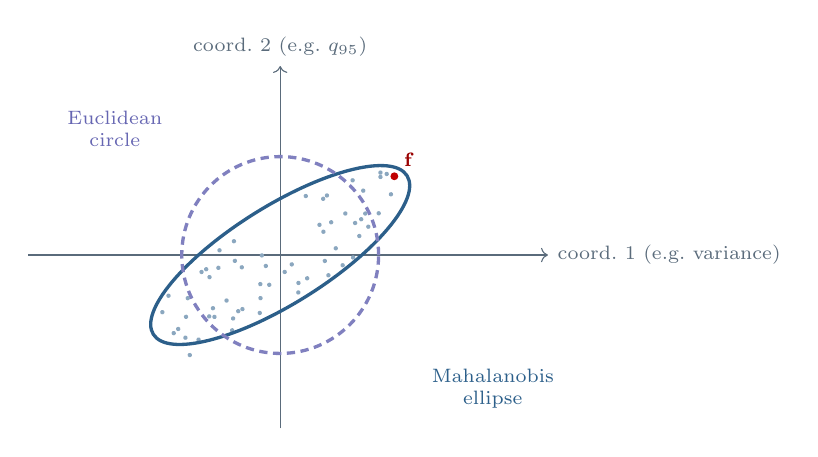
\begin{tikzpicture}[scale=1.0, font=\small]
  \draw[->, soft] (-3.2,0) -- (3.4,0) node[right]{\scriptsize coord.\ 1 (e.g.\ variance)};
  \draw[->, soft] (0,-2.2) -- (0,2.4) node[above]{\scriptsize coord.\ 2 (e.g.\ $q_{95}$)};
  % correlated cloud (tilted ellipse of points)
  \begin{scope}[rotate=32]
    \foreach \i in {1,...,60}{
      \pgfmathsetmacro{\rx}{1.7*rand}
      \pgfmathsetmacro{\ry}{0.55*rand}
      \fill[accent!55] (\rx,\ry) circle (0.028);
    }
    % Mahalanobis equidistance ellipse
    \draw[accent, very thick] (0,0) ellipse (1.9 and 0.62);
  \end{scope}
  % Euclidean circle (same Euclidean radius)
  \draw[NavyBlue!50, very thick, densely dashed] (0,0) circle (1.25);
  % a test point
  \fill[red!75!black] (1.45,1.0) circle (0.05) node[above right, red!60!black, font=\scriptsize]{$\fvec$};
  \node[accent, font=\scriptsize, align=center] at (2.7,-1.7) {Mahalanobis\\ellipse};
  \node[NavyBlue!60, font=\scriptsize, align=center] at (-2.1,1.6) {Euclidean\\circle};
\end{tikzpicture}
\\[-0.1em]
{\scriptsize The point $\fvec$ lies \emph{inside} the Euclidean circle (looks normal) but
\emph{outside} the Mahalanobis ellipse (is anomalous), because it departs along the thin axis where
the normal data barely varies. Euclidean misses it; Mahalanobis catches it.}
\end{center}

\subsection{The covariance is additive too --- closing the loop}

The reference $(\boldsymbol{\mu}, \Cov)$ is itself built from additive carriers, exactly as in \S1,
now lifted from scalars to vectors. With the vector power sums
\begin{equation}
  \mathbf{P}_1 = \sum_i \fvec_i \in \R^9,
  \qquad
  \mathbf{P}_2 = \sum_i \fvec_i \fvec_i^{\top} \in \R^{9\times 9},
\end{equation}
both sums-of-per-element-functions and hence additive (Theorem~\ref{thm:add}, componentwise), the
estimates are $\boldsymbol{\mu} = \mathbf{P}_1 / n$ and
$\Cov = \mathbf{P}_2 / n - \boldsymbol{\mu}\boldsymbol{\mu}^{\top}$. So the model a future
Mahalanobis detector needs is a \emph{small, mergeable summary} --- a vector and a $9\times 9$ matrix
--- maintainable over the same bitemporal, distributed rails as everything else. The additivity
thread of \S1 reaches all the way to \S3.

\subsection{Why Mahalanobis beats nearest-neighbour / ANN \emph{for this question}}

It is tempting to reach for a nearest-neighbour approach: store all historical fingerprints, and flag
the current one if its distance to the nearest stored example is large --- with approximate
nearest-neighbour (ANN) indexing to keep search fast at scale. For the \emph{anomaly-scoring}
question (``is this instrument abnormal versus its own normal?''), Mahalanobis is the better fit, for
four reasons.

\begin{enumerate}[leftmargin=1.5em, itemsep=0.35em]
  \item \textbf{It models ``normal'' directly.} Mahalanobis scores distance from the \emph{centre} of
        normal, shaped by normal's \emph{covariance} --- yielding a calibrated ``how many SDs out''
        with a clean statistical meaning (\S3.2). A nearest-neighbour distance means ``how close is
        the single most similar past example,'' which depends on how densely that region was sampled
        and has no comparable statistical interpretation.
  \item \textbf{It needs a summary, not a corpus.} Mahalanobis requires only
        $(\boldsymbol{\mu}, \Cov)$ --- a tiny, additive, mergeable object (\S3.3). Nearest-neighbour
        requires retaining the \emph{whole history} of fingerprints and an index over them; the
        memory and maintenance cost grows with the data, and the index is not additive.
  \item \textbf{It is exact and index-free.} Scoring is one quadratic form, $O(d^2)$ with $d=9$ ---
        trivial, and \emph{exact}. ANN exists precisely because exact nearest-neighbour search is
        expensive in high dimensions; it trades accuracy for speed and adds index structures
        (HNSW, IVF) that are overkill for a nine-dimensional per-instrument score.
  \item \textbf{It is correlation-aware by construction.} A raw-space nearest-neighbour search
        inherits the scale and correlation pathologies of \S3.1 unless you \emph{first} whiten --- but
        whitening requires the covariance, at which point the parametric Mahalanobis-to-centre is
        simpler and more interpretable than searching neighbours in whitened space.
\end{enumerate}

\begin{tcolorbox}[keybox, title={Two different questions --- be precise about which}]
Mahalanobis and ANN are not competitors so much as answers to different questions.
\textbf{Mahalanobis} answers \emph{``is this instrument abnormal relative to its own normal?''} ---
parametric anomaly scoring against a single, unimodal centre, needing only $(\boldsymbol{\mu},\Cov)$.
\textbf{Nearest-neighbour / ANN} answers \emph{``which other instruments are most similar to this
one?''} --- nonparametric retrieval over a large fleet of vectors, where an index genuinely earns its
keep. The first is the drift/anomaly question of this project; the second is the
cross-instrument-similarity question deliberately fenced as future work. Choosing Mahalanobis for the
first is not a rejection of ANN --- it is using each where it is correct.
\end{tcolorbox}

\subsection{An honest caveat: estimating the covariance}

Mahalanobis is only as good as $\Cov^{-1}$, and a $9 \times 9$ covariance has $45$ free parameters.
Estimated from too few fingerprints, $\Cov$ is noisy or singular and $\Cov^{-1}$ amplifies that noise.
Three standard mitigations apply, in increasing order of caution: (i) require enough reference
samples before trusting the full matrix; (ii) use \emph{shrinkage} (e.g.\ Ledoit--Wolf), pulling the
estimate toward a well-conditioned target; or (iii) fall back to a \emph{diagonal} covariance ---
per-coordinate standardisation only --- which still fixes the scale problem of \S3.1 even if it
ignores correlations. This is a deployment detail, not a flaw in the choice: it is named here so the
future work begins with eyes open.

\section*{Closing}
\addcontentsline{toc}{section}{Closing}

One idea has carried the whole document. The statistics worth keeping are \emph{sums of per-element
functions}; such sums form a commutative monoid; and that single algebraic fact is what lets the
system merge summaries across time and across machines, recover exact moments without bias, and ---
lifted from scalars to vectors --- maintain the very covariance a future Mahalanobis detector would
need. Around that spine sit two geometric choices: measuring distribution drift by the
ground-distance-aware, physically-interpretable Wasserstein distance rather than the bin-wise
divergences that are blind to it; and, when the time comes to compare fingerprints, measuring
abnormality by the scale- and correlation-aware Mahalanobis distance rather than by nearest-neighbour
search that answers a different question.

This was the seed: a small piece of mathematics that wanted to be built. The rest of the project is
that seed, grown.

\vfill
\begin{center}
{\color{soft}\rule{0.4\textwidth}{0.4pt}}\\[0.4em]
{\scriptsize\color{soft} BinMoments --- Mathematical Companion. Architecture by the author;
implementation AI-assisted.}
\end{center}

\end{document}
